\documentclass[tikz,border=2pt]{standalone}
\usepackage{amsmath,amssymb}
\usepackage{tikz}
\usetikzlibrary{arrows.meta}

\begin{document}
% The max flow problem as an LP: variables x_ij per edge, maximise the flow leaving the
% source, with capacity bounds and one conservation equation per intermediate vertex.
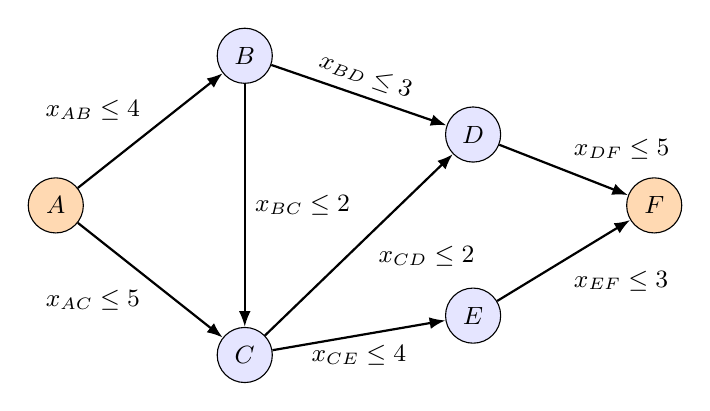
\begin{tikzpicture}[every node/.style={font=\small}, >={Latex[length=2mm]}, v/.style={draw, circle, fill=blue!10, minimum size=7mm, inner sep=0pt}]
	\node[v, fill=orange!30] (A) at (0,0) {$A$};
	\node[v] (B) at (2.4,1.9) {$B$};
	\node[v] (C) at (2.4,-1.9) {$C$};
	\node[v] (D) at (5.3,0.9) {$D$};
	\node[v] (E) at (5.3,-1.4) {$E$};
	\node[v, fill=orange!30] (F) at (7.6,0) {$F$};
	\draw[->, thick] (A) -- (B) node[midway, above left] {$x_{AB}\le4$};
	\draw[->, thick] (A) -- (C) node[midway, below left] {$x_{AC}\le5$};
	\draw[->, thick] (B) -- (C) node[midway, right] {$x_{BC}\le2$};
	\draw[->, thick] (B) -- (D) node[midway, above, sloped] {$x_{BD}\le3$};
	\draw[->, thick] (C) -- (D) node[pos=0.55, below right] {$x_{CD}\le2$};
	\draw[->, thick] (C) -- (E) node[midway, below] {$x_{CE}\le4$};
	\draw[->, thick] (D) -- (F) node[midway, above right] {$x_{DF}\le5$};
	\draw[->, thick] (E) -- (F) node[midway, below right] {$x_{EF}\le3$};
	\end{tikzpicture}
\end{document}
